\section{Background and Motivations}
\label{sec:bg}

In this section, we first provide the necessary background on distributed training
and motivate our selection of parameter server-based asynchronous training 
(Section~\ref{subsec:ddl}).  We then explain the opportunities and challenges
presented by training with transient servers (Section~\ref{subsec:transient}).
An overview of transient-based distributed training is illustrated in
Figure~\ref{bg:dist_train}.  
%Last, we describe our key research questions and
%summarize the empirical measurements  that shed light on future redesigns of 
%distributed deep learning frameworks. 


\subsection{Distributed Deep Learning}
\label{subsec:ddl}

In this paper, we focus on evaluating distributed training with parameter
server-based asynchronous training due to its popularity and potential
resilience to training server failures.  The concept of distributed deep
learning on multiple GPU servers is relatively new~\cite{jeffdean}, and a
number of frameworks such as TensorFlow~\cite{tensorflow} and
FireCaffe~\cite{firecaffe} have started to support training DNN models using
clusters of GPU servers. Note that this
approach is different from training on a single server with multiple GPUs. 


Conceptually, the training of a convolutional neural network can be divided
into four phases.
%, regardless of the number and type layers.  
First, the model parameters are initialized, often randomly or with a popular function such as
Xavier~\cite{glorot2010understanding}.  Second, one batch of input data  is
selected and the feed-forward computation is performed at each layer $l$ by
applying the function on the weights, inputs, and the bias term from the
previous layer $l-1$. The computation stops when the output layer is reached
and the results are recorded.  This second phase is identical to
the process of generating predictions using a trained model.  Third, model
errors are calculated by comparing the probability distribution (i.e., the
model output) generated for each input  to the known  true value and
multiplying by the derivative of the output layer. The errors are then
propagated from layer $l$ to its previous layer $l-1$ until reaching the first
layer.  Fourth, the model parameters between layer $l-1$ and layer $l$ are
updated by multiplying the learning rate and the gradient of layer $l$ and
weights at layer $l-1$. 



%%Input to  phase 2
%For each step, a subset of data is
%randomly chosen from the entire training dataset. Given this, there is a slight
%chance that some data will never be used for each epoch, regardless of whether
%it is single-GPU server or GPU cluster training. 



As the model gets bigger---i.e., more parameters and computation-intensive
layers---the training time also increases.  To speed up the training process,
phases two through four above can be distributed across different servers
to parallelize training.  A common way to do so is to have a parameter
server~\cite{stale1,geeps} that is in charge of updating model parameters (phase
four), and a cluster of powerful GPU servers to work on the forward and
backward propagation (phases two and three).  It is worth noting that phase two is
the most time-consuming of the training process~\cite{efficient_dnn} and, therefore, would enjoy the
largest benefit from adding more GPU servers.

In this paper, we adopt the asynchronous distributed training architecture
depicted in Figure~\ref{bg:dist_train}. Here  each worker keeps an entire copy
of the model and independently calculates gradients using its local copy of the
input data---this also referred to data-parallelism.\footnote{For training with
large volumes of data, the data are also often divided into shards.} In
addition, each worker can pull the most-recent model parameters from a
parameter server without needing to wait on the parameter server to collect and
apply gradients from all other workers, i.e., asynchronous training. It is also
possible to use more than one parameter server, in which case each worker
needs to contact all parameter servers (not depicted in the figure).
Consequently, workers might be working on slightly outdated models (indicated
by different shades in Figure~\ref{bg:dist_train}); this model staleness can
lead to a reduction of model accuracy. Currently, in TensorFlow distributed
training, one master worker will also periodically save the model parameters in
a process called \emph{model checkpointing}.
Even if one of the workers fails---e.g., the last worker colored with red in
Figure~\ref{bg:dist_train}---the training can still progress, albeit at a
degraded speed. However, if the master fails, the distributed training
also fails because we will not have access to the model files with the
converged accuracy. 


\begin{figure}[t]
\centering
    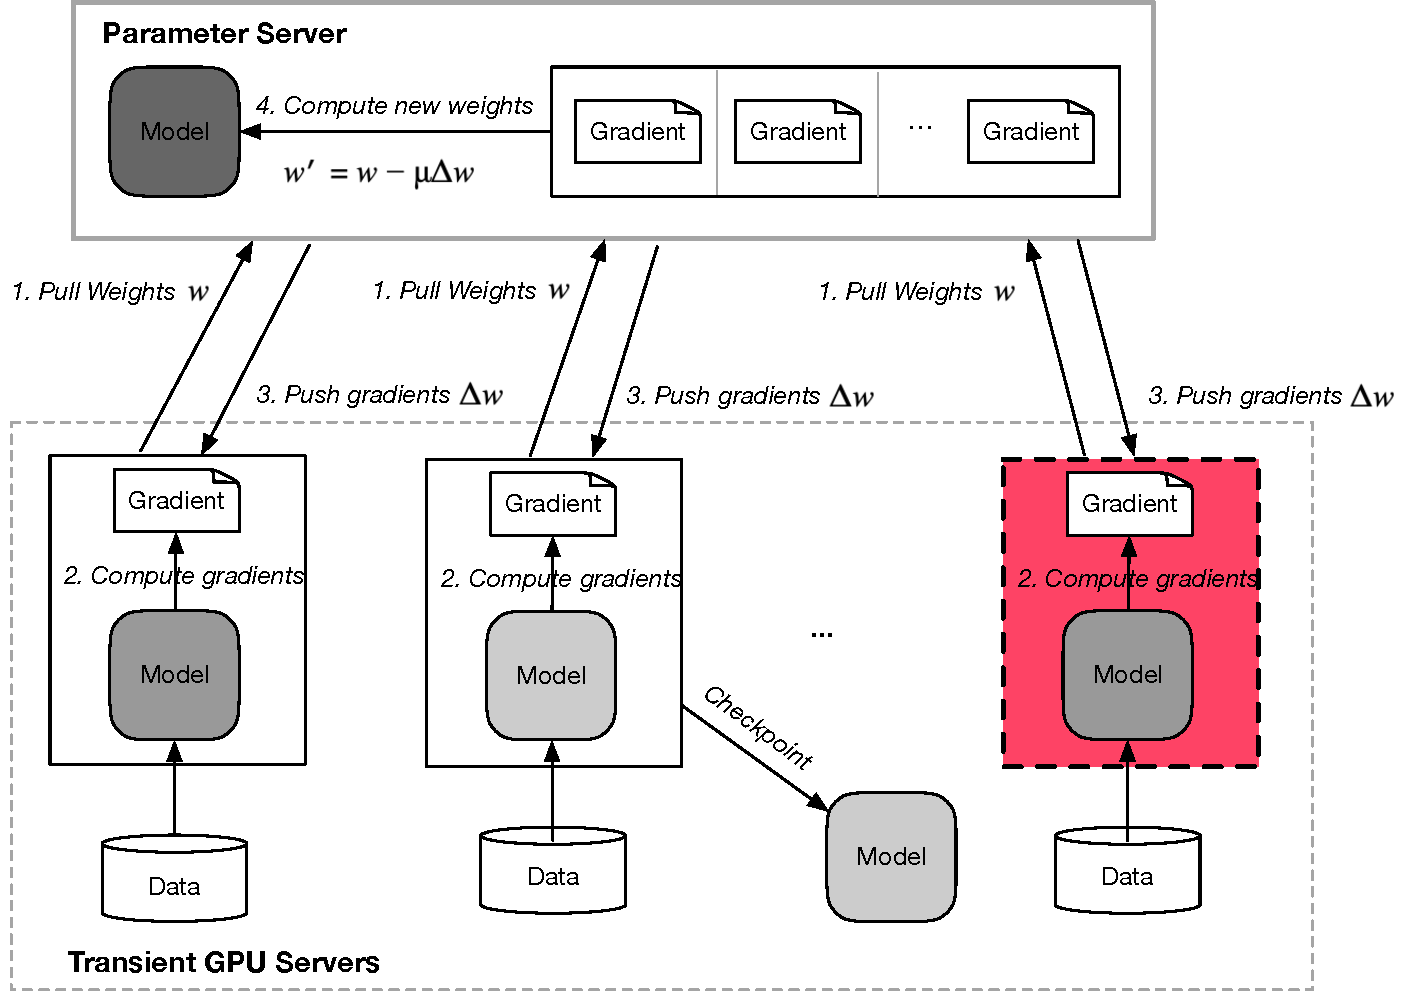
\includegraphics[width=0.96 \columnwidth ]{distributed_training.pdf}
\caption{\textbf{Illustration of distributed training on transient GPU
  servers.} We adopt an asynchronous distributed training architecture. The
  parameter server  runs on an on-demand CPU server and the workers (including a
  special master that is in charge of model checkpointing) run on transient GPU
  servers. Workers are in charge of calculating the gradient updates while the
  parameter server incorporates the gradients to update the model parameters.
  The training can still progress even if some of the workers (denoted in red)
  are revoked by the provider.}
    \label{bg:dist_train}
\end{figure}


\subsection{Transient Servers}
\label{subsec:transient}

\emph{Transient servers} are cloud servers that are offered at discounted
prices (up to 90\% cheaper). Major cloud providers, such as Amazon EC2 and
Google Compute Engine (GCE), offer transient servers in the form
of \emph{spot instances} and \emph{preemptible VMs}, respectively. Unlike traditional \emph{on-demand}
servers, cloud providers can revoke transient servers at any
time~\cite{ec2_spot,gce_preemptible}. When such situations arise, customers are
only granted a short time window---30 seconds for GCE and 2 minutes for
EC2---before permanently losing access to the server. This is often referred to
as \emph{server revocation}.

Aside from revocation, transient servers offer the same performance as
equivalently configured on-demand servers. For example, the training
performance with \emph{4 K80 transient} servers when \emph{r=0} (no
revocations) and training with \emph{4 K80 on-demand} servers are almost
identical, see Table~\ref{intro:tbl:motivation}.
  

Cloud transient servers exhibit three key characteristics that make them both
beneficial and challenging to leverage for distributed training. 

% static and dynamic pricing 
First, transient servers are significantly cheaper allowing customers to devote
additional servers to training, speeding up the training time while remaining
within a fixed monetary budget.  Depending on whether the transient servers are
statically priced (e.g, GCE preemptible VMs) or use a more dynamic pricing
model (e.g., Amazon spot instances), cloud customers have a range of possible
cluster configurations  that may evolve over time. For instance, in the case of
dynamic pricing, cloud customers may want to regularly monitor prices and
adjust the number and type of servers to maximize training performance and reduce
costs.


Second, the availability of transient servers, compared to their on-demand
counterparts, can be lower or even unpredictable.  Here the availability of
cloud servers refers to the probability of cloud providers fulfilling the
resource request in a timely manner. 
%As reported in~\cite{amazonnews, spotlight}, as transient servers become more
%popular and the demand for them grow rapidly in the past few years (exceeding
%the requests to on-demand servers in 2012), customers who would want to launch
%transient servers might not even quickly get the resources. 
Availability depends, in part, on the overall demand for servers (both
on-demand and transient) in the local region~\cite{spotlight}.  Therefore, to
best utilize transient servers it is likely that customers will need to request
servers with different (but more available) resource capacities and from multiple regions.

%  voluntary and forced revocation due to different lifetimes 
Third, transient servers have uncertain lifetimes. Here a server's
\emph{lifetime} is
the time interval  between when the cloud provider satisfies the customer's
request for a new server and the time the server is revoked. Different cloud
providers have different policies that directly affect server lifetimes. For
Google Compute Engine, the maximum lifetime of any transient server is at  most
24 hours. That is, even though GCE preemptible VMs can be revoked at any point, 
they are guaranteed to be revoked after 24 hours. 

We empirically measured the lifetime of GCE transient servers (with the
configurations detailed in Table~\ref{tbl:exp_setup}). Our measurement involves 
more than 600 transient servers that were requested at different times, from 
different data center locations, and with different levels of resource utilization. 
In Figure~\ref{design:gpu_lifetime}, we compare the lifetimes of GCE transient 
servers. We observe that different GPU servers have different revocation
patterns. Further we find that 
even though approximately 70\% of servers live the full 24 hours, about 20\% are revoked 
within the first two hours---in the latter case, distributed training that lasts more than two hours 
will be subject to revocation impacts. 

%We observe that although some transient servers can live up to 24 hours, about XX\% of them are revoked
%within the first two hours. Further, more powerful GPU servers experience more
%revocations earlier. 

In summary, cloud transient servers present an opportunity to speed up deep
learning with cheaper server resources.  However, considering the potential
revocations and unavailability of transient servers, leveraging these resources
requires us to rethink existing techniques for distributed training.  Current
distributed frameworks, designed with stable on-demand servers in mind, do not
adequately support the features that are necessary for leveraging transient
servers; e.g., dynamic cluster adjustment, robust model checkpointing, 
or support for heterogeneous and geographically distributed clusters. 


    
 \begin{figure}[t]
\centering
    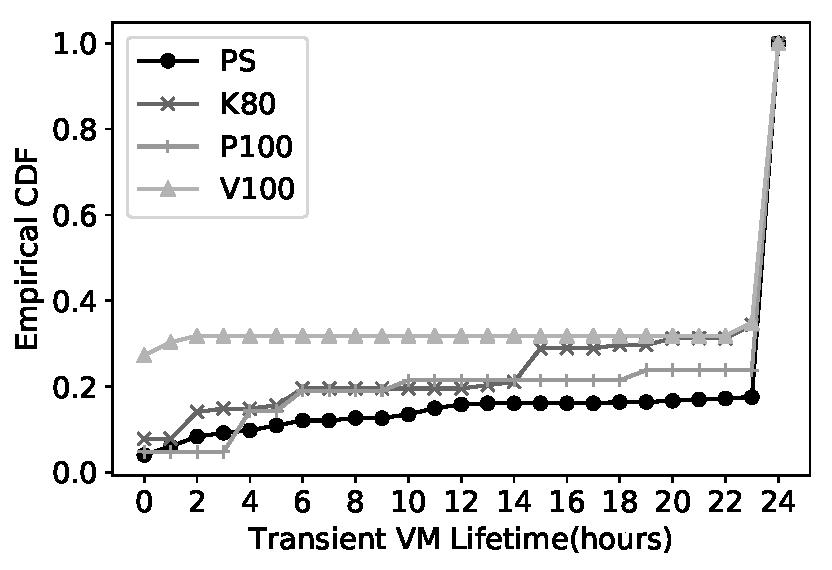
\includegraphics[width= 0.88 \columnwidth ]{lifetime_new.pdf}
\caption{\textbf{CDF of Google preemptible GPU server lifetimes.} We measure
   the lifetime as the time between when a preemptible GPU server is ready
   to use and when the server is revoked by the Google cloud
   platform. Note that Google transient servers have a maximum lifetime of 24
   hours. We observe that less than 20\% of transient servers are revoked in
   the first two hours.}
%   and then additional 10\% can almost live up to the maximum of 24 hours.}
    \label{design:gpu_lifetime}
\end{figure}
